
\section{Foundation Model Intro}

% What is the problem: training a model that allows people to quickly finetune on their own insertion task
Models that are pre-trained on broad datasets and can be fine-tuned to specific problems, sometimes called ``foundation models'' have driven recent progress in vision and NLP.
For instance, bidirection encoders from transformers (BERT) ~\cite{devlin2019bert} pretrained on large language datasets (100Ms of sentences) is now the standard starting point for fine-tuning to language models on custom language tasks and on custom data of much smaller size (10,000s of sentences).
This type of pretraining capability enables machine learning to be used to solve more bespoke problems, greatly widening the applicability of ML methods to real-world applications.
Similarly, robotics applications are often narrow, so the ability to utilize broad prior data but fine-tune on a specific task would be extremely valuable.
However, in robotics, such data sharing and model sharing have proven to be relatively difficult.

% Why is interesting and important
% But if trained, such a model that could be fine-tuned for a particular setting would benefit any entity solving robotic insertion tasks.

% Why is it hard 
Using foundation models in RL runs into many challenges: robots have different controllers, action spaces, different proprioceptive inputs, different image properties (resolution). Unlike vision and language, robotics data is also more siloed: the backgrounds and morphologies are repeated across many trajectories, so the data is not very diverse along these axes. In light of these differences, what module should actually be shared?

% Our solution
We propose to share data across multiple robots by a combination of representation learning and offline RL followed by finetuning. The representation learning has to be done carefully to enable sharing of perception and task information while having individual representations for each embodiment. Our model, which consists of a unique encoder per robot controller, but shared latent variables for everything else, is shown in Figure 1~\ref{fig:gm}. We use offline reinforcement learning with implicit Q-learning (IQL) across multiple datasets to initialize a policy based off of this learned representation. Then on a new task, we train a new controller embedding if necessary, then fine-tune with IQL.

% Main contributions
The main contribution of this paper is to show that by leveraging large datasets for insertion, we can get positive transfer to inserting new connectors on new robots.
More broadly, we envision this as a recipe for broader robot control tasks. Insertion is unique in that the visual features shared between different tasks for control are clearly shared: aligning edges, corners, angles of connectors, and so on. Thus insertion is a good starting point for foundation model research in robotics. We inspect the learned features in Section <> by visualizing what parts of the image the network is paying attention to.

\begin{figure}[t]
    \centering
    \begin{subfigure}[b]{0.99\linewidth}
        \center
        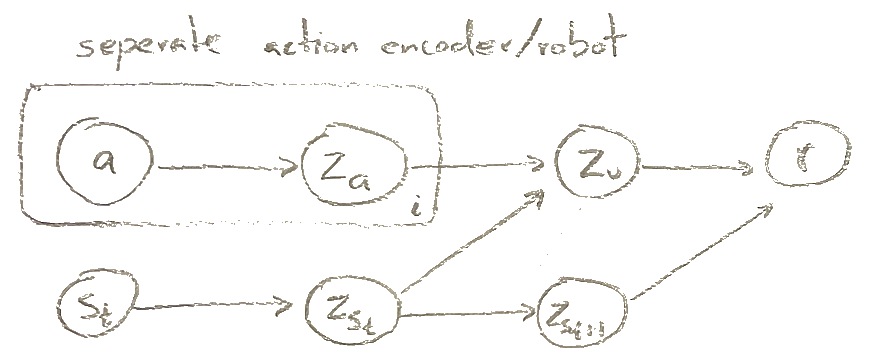
\includegraphics[width=0.9\textwidth]{imgs/pgm.png}
    \end{subfigure}

    \caption{Graphical model for extracting re-usable representations from multi-robot insertion datasets. Robot-specific action encoders $p(z_{a_i}|a_i)$ are learned separately for each robot. All other latent representations are shared: a state encoder $p(z_{s_t}|s_t)$ and a common action encoder $p(z_u|z_a, z_{s_t})$ which is conditioned on the state in order to provide enough context to represent actions globally. The representations can be trained using a combination of dynamics predictions (inverse or forward), contrastive objectives, and offline reinforcement learning. }

    \label{fig:gm}
    \vspace{-0.5cm}
% \end{wrapfigure}
\end{figure}


\section{OLD Introduction}

% What is the problem
% Industrial insertion 
Industrial insertion tasks, such as inserting plugs in sockets and setting screws, are accomplished in factories today with specialized control algorithms.
%%SL.12.28: I assume you mean are performed by robots? While it's true that people setting screws and inserting plugs use "specialized control algorithms," that seems like a rather unconventional way to describe it ;)
These algorithms are often brittle and unreliable, requiring perfect precision to perform well; once a small amount of uncertainty or variability is introduced, they often fail.
%%SL.12.28: This one might be a triggering sentence for a lot of good old fashioned robotics people
% There is a large family of industrial insertion tasks, such as inserting plugs in sockets, setting screws, and many more.
This brittleness means that in many manufacturing situations, we are still not able to automate these processes, instead requiring humans to be involved in the manufacturing process.
If we had sufficiently robust algorithms that dealt with significant sources of variance successfully, we could automate many tasks that must be completed manually today.
% Common approaches to automate them today involves a robot engineer spending potentially 100+ hours designing a custom solution to a specific task.
% But this does not scale; only very common tasks can be solved this way. 
% Instead, if we were able to allow robots to quickly acquire skills in a new setting, they could be used much more widely.

% Why is it interesting and important
% Very useful in terms of economic value, lots of different tasks that look similar

% Why is it hard
% Generalization in robotics, sharing knowledge between tasks
% One major challenge is the diversity of these tasks, so learning methods are a good fit.
Such an algorithm must be general enough to handle many different tasks with the same input modality, capable of sharing insertion strategies between various scenarios. 
%%SL.12.28: It's not actually obvious why this is true
Deep reinforcement learning holds the promise of learning control policies from large amounts of data and rich observations such as images, and has been shown to do so in simulated domains.
But thus far, deep reinforcement learning has not shown generalization for robotics manufacturing tasks in the real-world.
Such a system would require performant offline RL and large, diverse datasets to learn from.
%%SL.12.28: I wonder if we can have a somewhat more nuanced opening -- right now, the first two paragraphs basically say: normal control sucks, RL will fix it. That's kind of a bold statement, but perhaps too inflamatory, and perhaps too lacking in nuance. I wonder if we can have some motivation that is a bit more specific to what our method is actually doing specifically.

Furthermore, perfect zero-shot to every possible task is an onerous requirement even with coverage over many tasks.
Instead, if an algorithm could be fine-tuned to a specific task with relatively little additional data, the burden of initial performance is much lower.
Such a learning protocol could additionally be used to collect data on successively more complicated tasks, enabling lifelong learning of more and more diverse skills.
%%SL.12.28: This part is probably more important, but the motivation beforehand needs to get at this point more directly, otherwise this paragraph reads a bit like an afterthought.

% Unique solution
% Self-supervised life-long learning on large family, demonstrating transfer
In this paper, we focus on collecting and utilizing large datasets through lifelong self-supervised reinforcement learning for the purpose of generalization.
We require learning from large datasets to see transfer between different tasks - we show that we actually see this transfer in action.
We require learning from images to have the potential, with enough information/context, to generalize.
The data needs to be collected in a lifelong way to get high quality data, as opposed to prior robotics datasets with random actions \cite{dasari2019robonet}.
%%SL.12.28: The lifelong part is reasonable, but it needs to be motivated more effectively, and the experimental results need to actually back this up.
% It needs to be self-supervised to avoid having a human in the loop for reward supervision.

% Contributions
% Demonstrating real-world transfer and speeding up learning between different tasks
The main contribution of this paper is to show that lifelong reinforcement learning can enable generalization in industrial insertion tasks.
%%SL.12.28: It would be great if we can show this! Though it is a bit of a bold statement, it will set a high bar for the experimental results.
We show that new tasks can be learned within X trials, given our dataset of off-policy data from Y prior tasks of Z trajectories.
Our dataset will be made public at <URL>.
